\subsubsection{First Iteration}
As things currently stand, the gateway is able to receive transmissions from the Arduino, but the Arduino is unable to receive the acknowledge that the gateway sends upon OTAA.
However, the gateway is receiving data from the Arduino, and forwarding said data to The Things Network, where it is accessible.
We can see the Arduino's attempts at establishing a connection in \cref{fig:gateway_serial}.
\begin{figure}[ht]
  \centering
  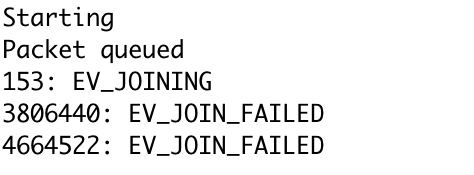
\includegraphics{figure/gateway_serial}
  \caption{The Arduino's attempts to establish a connection in the network.  Because it is not receiving the gateway's ACK signal, it is viewing its attempts as failures.}
  \label{fig:gateway_serial}
\end{figure}

However, we can see that the gateway is receiving the data that the Arduino is transmitting, because the data are appearing on The Thing Network's console.
The gateway's input and output are shown together in \cref{fig:gateway_console}, while only the data received from the Arduino are shown in \cref{fig:arduino_console}.
\begin{figure}[ht]
  \centering
  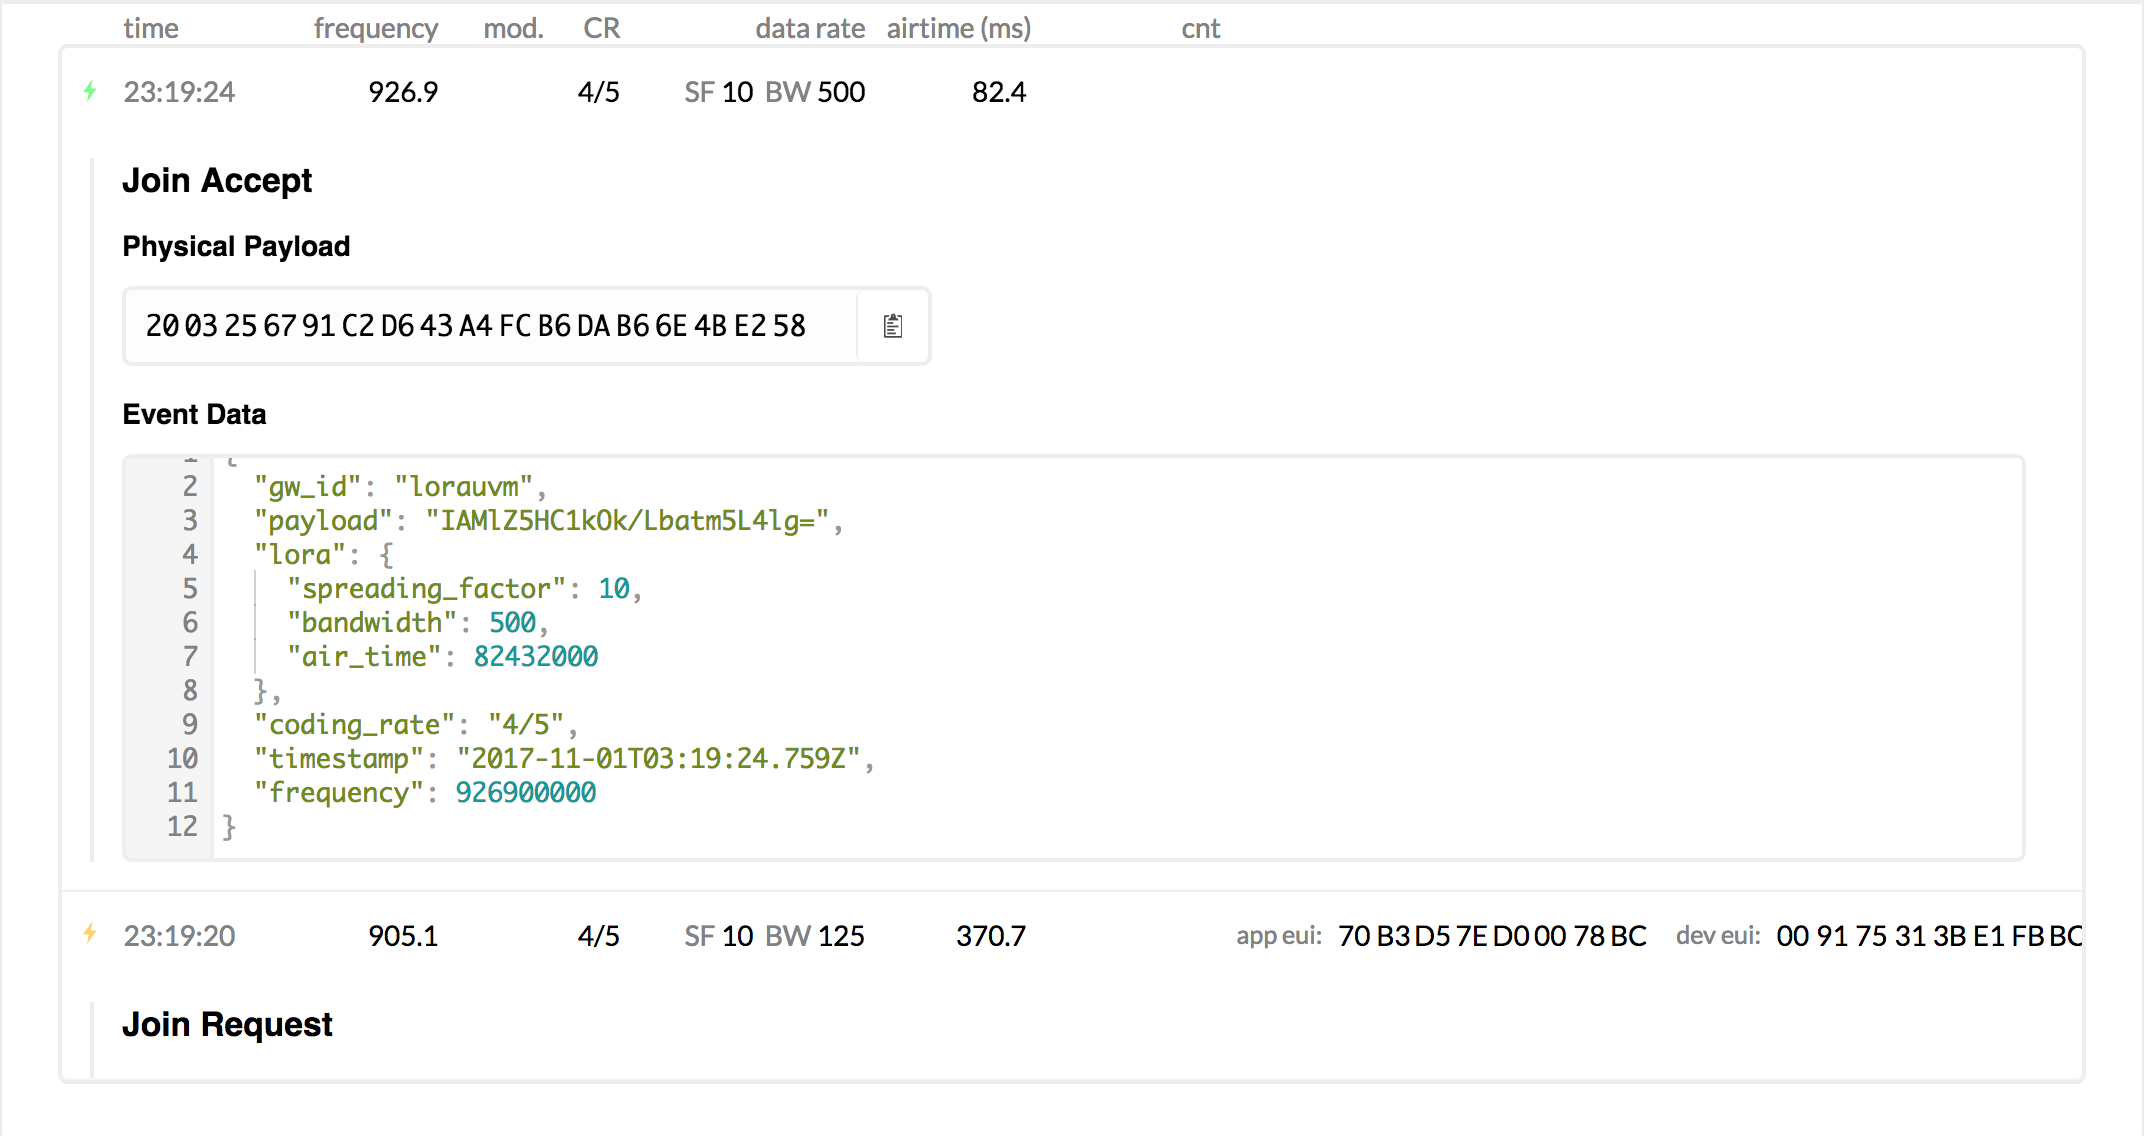
\includegraphics[width=\textwidth]{figure/gateway_console}
  \caption{The data received and transmitted by the gateway, as they appear on The Things Network's console.}
  \label{fig:gateway_console}
\end{figure}
\begin{figure}[ht]
  \centering
  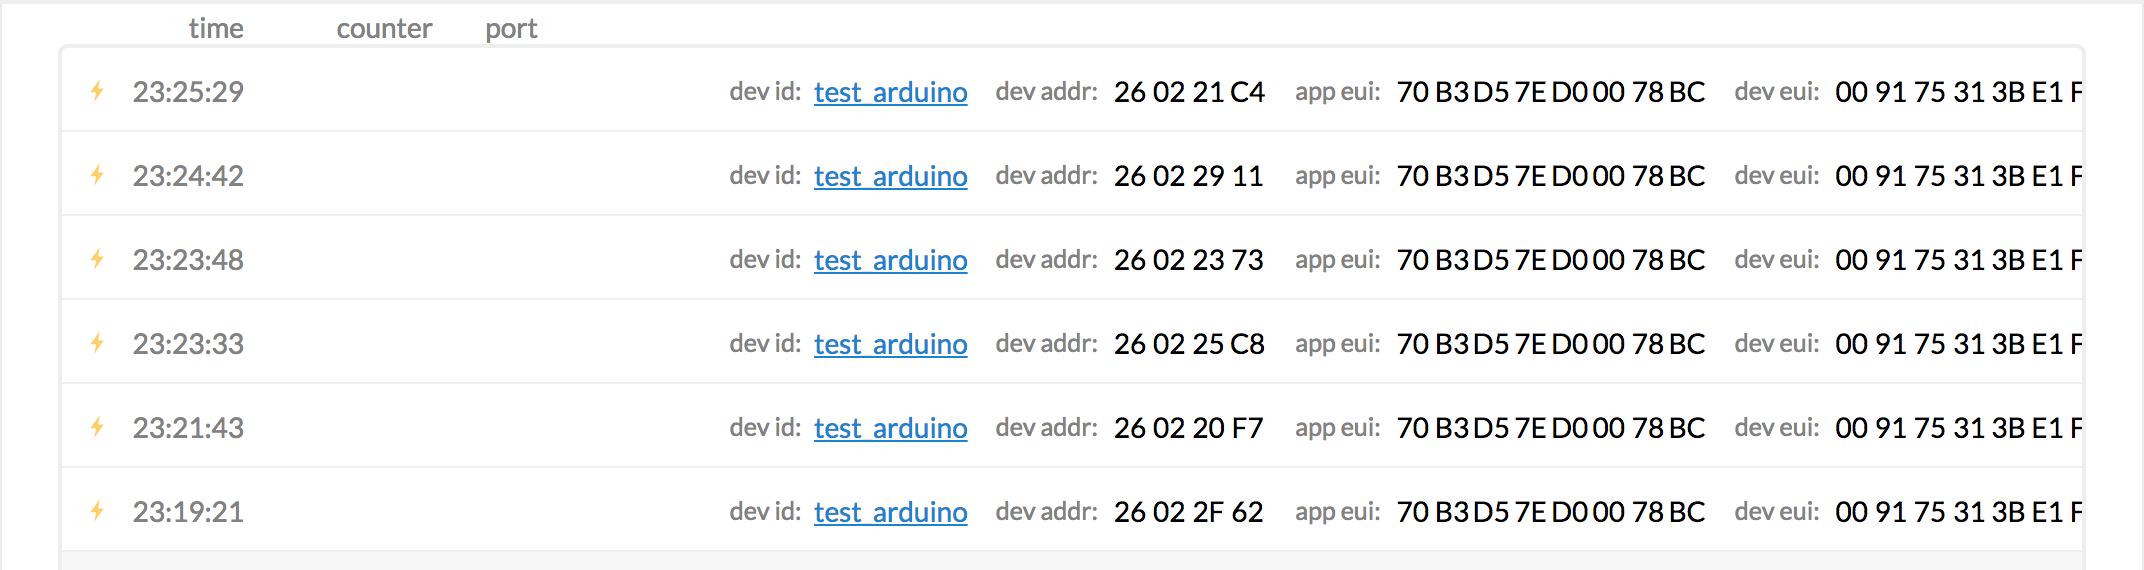
\includegraphics[width=\textwidth]{figure/arduino_console}
  \caption{The data transmitted by the Arduino, as they appear on The Things Network's console.}
  \label{fig:arduino_console}
\end{figure}

\subsubsection{Second Iteration}
After much troubleshooting, the Arduino was able to receive the acknowledge from the gateway.
This was achieved by changing the tolerance on the Arduino's clock, adding
\begin{lstlisting}[language=C++]
  LMIC_setClockError(MAX_CLOCK_ERROR * 1 / 100);
\end{lstlisting}
to the OTAA script's \lstinline[language=C++]{setup} function.
This allowed for a stable connection.

The issue with this connection is that the range is extremely limited, with a maximum of approximately \SI{20}{\meter}.

%%% Local Variables:
%%% mode: latex
%%% TeX-master: "../writeup"
%%% End:
